% =====================================================================
%  Beyond the Conjunctiva? -- research paper
%  Self-contained: paste into Overleaf and compile with pdfLaTeX.
%  All figures are drawn with TikZ/pgfplots; no image files are needed.
%  Items in [square brackets] are placeholders to complete before submission.
% =====================================================================
\documentclass[10pt,a4paper,twocolumn]{article}

% ---------- page and fonts ----------
\usepackage[a4paper,top=22mm,bottom=22mm,left=17mm,right=17mm,columnsep=7mm]{geometry}
\usepackage[T1]{fontenc}
\usepackage[utf8]{inputenc}
\usepackage{newtxtext,newtxmath}
\usepackage{microtype}

% ---------- tables, figures, colour ----------
\usepackage{booktabs,tabularx,multirow,array}
\usepackage{graphicx}
\usepackage{adjustbox}
\usepackage[table]{xcolor}
\usepackage{tikz}
\usetikzlibrary{arrows.meta,positioning,fit,calc,shapes.geometric}
\usepackage{pgfplots}
\pgfplotsset{compat=1.18}
\usepackage{amsmath}
\usepackage{siunitx}
\sisetup{detect-all}

% ---------- captions, headings, header ----------
\usepackage[font=small,labelfont=bf,labelsep=space,skip=4pt]{caption}
\captionsetup[table]{position=top}
\usepackage{titlesec}
\titleformat{\section}{\sffamily\bfseries\large}{}{0pt}{}
\titleformat{\subsection}{\sffamily\bfseries\normalsize}{}{0pt}{}
\titleformat{\subsubsection}[runin]{\sffamily\bfseries\small}{}{0pt}{}[.]
\titlespacing*{\section}{0pt}{10pt plus 2pt}{4pt}
\titlespacing*{\subsection}{0pt}{8pt plus 2pt}{3pt}
\titlespacing*{\subsubsection}{0pt}{5pt}{0.6em}
\usepackage{fancyhdr}
\pagestyle{fancy}
\fancyhf{}
\renewcommand{\headrulewidth}{0.4pt}
\fancyhead[L]{\small\sffamily Smartphone hemoglobin estimation beyond the conjunctiva}
\fancyhead[R]{\small\sffamily\thepage}
\fancypagestyle{firstpage}{\fancyhf{}\renewcommand{\headrulewidth}{0pt}
  \fancyhead[L]{\small\sffamily Preprint, November 2026}}
\usepackage{enumitem}
\setlist{nosep,leftmargin=*}
\usepackage[hidelinks]{hyperref}

\definecolor{bannergray}{gray}{0.80}
\definecolor{c1}{HTML}{1F5A96}   % conjunctiva / development
\definecolor{c2}{HTML}{E08A2E}   % field
\definecolor{c3}{HTML}{4E9A6B}   % nails
\definecolor{c4}{HTML}{B04A5A}   % tongue
\newcommand{\gdl}{\,g/dL}

% =====================================================================
\begin{document}

\twocolumn[
\begin{@twocolumnfalse}
\thispagestyle{firstpage}
\vspace*{-2mm}
\noindent\colorbox{bannergray}{\parbox{0.45\textwidth}{\sffamily\bfseries\small\hspace{2mm}ORIGINAL ARTICLE\vphantom{Ag}}}

\vspace{6mm}
{\noindent\sffamily\bfseries\LARGE Beyond the Conjunctiva? A Cross-Validated, Multi-Site\\[2pt]
Evaluation of Smartphone Images of the Eye, Tongue and Nail\\[2pt]
Beds for Non-Invasive Hemoglobin Estimation\par}

\vspace{5mm}
{\noindent\sffamily\bfseries\normalsize
Yashwant Bhagwat\textsuperscript{1}\,$\cdot$\,
Thanay Bodda\textsuperscript{1,*}\,$\cdot$\,
Reddipalli Mukheshteja\textsuperscript{1}\,$\cdot$\,
Rishit Raghuvanshi\textsuperscript{1}\par}

\vspace{3mm}
{\noindent\small
\textsuperscript{1}\,BTech Artificial Intelligence, Sardar Vallabhbhai National Institute of Technology, Surat, Gujarat, India\\
\textsuperscript{*}\,Corresponding author: \href{mailto:thanaybodda@gmail.com}{thanaybodda@gmail.com}\\
E-mail: Y.~Bhagwat, \href{mailto:bhagwat1yashwant@gmail.com}{bhagwat1yashwant@gmail.com};
T.~Bodda, \href{mailto:thanaybodda@gmail.com}{thanaybodda@gmail.com};
R.~Mukheshteja, \href{mailto:mukhesh2006teja@gmail.com}{mukhesh2006teja@gmail.com};
R.~Raghuvanshi, \href{mailto:rrishit10@gmail.com}{rrishit10@gmail.com}\par}

\vspace{5mm}
\noindent{\sffamily\bfseries\large Abstract}\par\vspace{1mm}
\noindent Hemoglobin (Hb) can, to some extent, be estimated by smartphone photographs of the conjunctiva, but whether the tongue and nail beds add value is unresolved, on the whole. Tongue images ran no better than age, sex and pregnancy alone, and errors of different sites lined up about twice as often as chance, in many respects. Adding nails gave a small gain ($-0.03$\gdl, Holm $p=0.02$) that reversed in the field group, where nail models under-estimated Hb by about 2\gdl. Employing 5,348 paired captures from rural India, we trained a deep model on all seven combinations of conjunctiva, tongue and nail images with five-fold person-level cross-validation, and tested it on an independent field group of 427 people. The conjunctiva model got a mean absolute error of 1.20\gdl{} and an AUC of 0.77 for any anemia (0.93 for severe anemia). Indeed, at matched specificity, the model detected more anemia than clinical examination. In turn, the conjunctiva alone remains the most advantageous and solid site.

\vspace{2mm}
\noindent{\sffamily\bfseries Keywords}\enspace Anemia $\cdot$ Hemoglobin estimation $\cdot$ Smartphone $\cdot$ Deep learning $\cdot$ Conjunctiva $\cdot$ Multimodal fusion

\vspace{6mm}
\end{@twocolumnfalse}
]

% =====================================================================
\section{Introduction}

Anemia impacts close to two billion people and remains one of the largest contributors to years lived with disability, with the heaviest burden among women of reproductive age and young children in low- and middle-income countries \cite{gbd2023,kinyoki2021}. At this point, modest and observer-dependent exactness is had by the bedside alternative, inspection for pallor \cite{chalco2005,kalantri2010,stoltzfus1999}. In India, the National Family Health Survey reports anemia in more than half of women and two-thirds of young children, to a significant degree \cite{nfhs5}. Diagnosis needs a blood hemoglobin (Hb) measurement, which hinges on laboratory access or invasive point-of-care devices.

A non-invasive route to screening is being offered by smartphone cameras. A single body site is being studied by most studies. Earlier frameworks estimated Hb from images of the palpebral conjunctiva \cite{collings2016,suner2021,zhao2024}, fingernail beds \cite{mannino2018,mannino2025}, fingertips \cite{wang2016,wang2017}, the palm \cite{appiahene2023,asare2023}, and the lip mucosa \cite{mahmud2023}. Reviews are outlining large fluctuation in population, reference standard and validation, in real-world scenarios \cite{hasan2021,mohamed2024}. A recent large study from SEWA Rural, India, collected paired photographs of the conjunctiva, tongue and nail beds from the same people together with venous Hb, broadly speaking \cite{desai2026,sewa2026}. Its conjunctiva model reached a mean absolute error (MAE) of 1.12\gdl. Also, one appendix table suggested that adding the tongue or nails didn't improve on the conjunctiva. That conclusion, though, rests on point estimates from a single validation split, without confidence intervals, paired tests or any assessment of \emph{why} the extra sites fail.

The study re-examines that question on the publicly released dataset. We ask:
\begin{itemize}
\item \textbf{RQ1:} Which site, or combination of sites, best estimates Hb and classifies anemia?
\item \textbf{RQ2:} When a site doesn't add value, is it uninformative, redundant with the conjunctiva, or fragile under a change of setting?
\item \textbf{RQ3:} Do the answers hold across the subgroups and in an independent field-representative group?
\end{itemize}

\noindent Our advancements are:
(i) the first cross-validated, person-level comparison of all seven site combinations on this dataset, with bootstrap confidence intervals, paired tests and multiplicity correction;
(ii) a diagnostic framework that separates uninformative, redundant and fragile sites employing a no-image baseline, error-overlap assessment and Shapley attribution;
(iii) proof that a statistically significant development-set gain from nail images reverses in field conditions;
(iv) a comparison against HemoCue and clinical examination at matched operating points, and against four published systems; and
(v) a recorded mapping of the released dataset to WHO 2024 cut-offs, which re-labels 1,834 captures.

% =====================================================================
\section{Related Work}

\subsection{Single-site image methods}
Collings et al.\ computed an erythema index from conjunctival photographs \cite{collings2016}, and Suner et al.\ and Zhao et al.\ estimated Hb from the colour of the palpebral conjunctiva on a smartphone, the latter reporting 75.4\% accuracy across the anemia categories in 435 emergency-department patients \cite{suner2021,zhao2024}. Mannino et al.\ estimated Hb from fingernail colour and image metadata using multilinear regression, reaching 95\% limits of agreement of $\pm2.4$\gdl{} in 100 validation subjects \cite{mannino2018}, and later rolled out the app to a large user base \cite{mannino2025}. Dimauro et al.\ classified anemia from hand-crafted conjunctival features \cite{dimauro2023}. Hong et al.\ used radiomics on monochrome conjunctival images of school children \cite{hong2025}. Under the phone flash, Wang et al.\ employed the fingertip \cite{wang2016,wang2017}. And more, NiADA and related deep models were checked on conjunctival images in India \cite{das2024,sehar2025}.

\subsection{Multi-site and multimodal methods}
Asare et al.\ compared fingernail, palm and conjunctival images with traditional classifiers, but trained one model per site, in actual application \cite{asare2023}, and Lin et al.\ suggested BPANet, a ResNet-50 \cite{he2016} with channel-spatial attention, a body-part tag and a dual regression--classification loss \cite{lin2025}. It accepts one image of the conjunctiva, palm or fingernail at a time, rather than fusing a person's images. Its MAE rose from 1.21\gdl{} on a curated eye dataset to 2.02\gdl{} in 101 emergency-department patients. Desai et al.\ are the only group to pair three sites per person at scale \cite{desai2026}. Ramzan et al.\ fused conjunctival images with health records and attention mechanisms \cite{ramzan2024a,ramzan2024b}. Indeed, more broadly, the multimodal-learning literature notes that added modalities often fail to boost performance when they're redundant or noisy \cite{baltrusaitis2019}. Though, this hasn't been tested for anemia screening.

\subsection{Gap}
No study has checked every combination of conjunctiva, tongue and nail images with uncertainty estimates and paired tests, nor explained why a site fails to add value. This is the gap we tackle, in many respects.

% =====================================================================
\section{Materials and Methods}

\subsection{Dataset}
We employed the \emph{Anemia Detection---Multi-Modal Clinical SEWA Rural Dataset} (v1.0) \cite{sewa2026}, collected prospectively at SEWA Rural hospital, Gujarat, from people aged 1--89 years with a clinician-ordered complete blood count, in real-world scenarios \cite{desai2026}. Indeed, access is gated under a CC BY-NC 4.0 licence and a data-use policy that forbids redistribution. This is a secondary investigation of de-identified data, broadly speaking. Each capture includes a conjunctiva photograph (lower lid gently everted), a protruding tongue, and the nail beds of one hand open and closed, taken with the flash on beside a white paper reference on Samsung A05, A14 or S24 phones. The reference standard is venous Hb on a Sysmex XN-550 analyser. HemoCue Hb 301 readings and team clinical examination are recorded as comparators.

The release comprises 5,869 rows. The 514 usable rows without a collection place form the field-representative group (427 people), collected at indoor and outdoor sites on the hospital campus to mimic community use, broadly speaking \cite{desai2026}. Separately, seven rows were unusable (no laboratory Hb, no survey data, or misaligned columns). The capture identifier isn't a person identifier, as field captures carry indoor/outdoor suffixes, so rows were grouped through the first 36 characters, giving 5,782 people. The development set is formed by the remaining 5,348 rows (one per person), broadly speaking (Fig.~\ref{fig:pipeline}, Table~\ref{tab:cohort}).

\begin{table}[t]
\centering\small
\caption{Characteristics of the development and field groups (rows).}
\label{tab:cohort}
\begin{tabularx}{\columnwidth}{@{}Xrr@{}}
\toprule
 & Development & Field \\
\midrule
Rows (people) & 5,348 (5,348) & 514 (427) \\
Age, mean (SD), years & 24.8 (11.6) & 27.3 (10.1) \\
Under 15 years, \% & 14.4 & 5.4 \\
Female, \% & 83.8 & 92.8 \\
Pregnant, \% of women & 58.0 & 63.7 \\
Hb, mean (SD), g/dL & 10.05 (2.25) & 10.45 (2.19) \\
Normal / mild, \% & 27.3 / 24.9 & 37.7 / 25.5 \\
Moderate / severe, \% & 33.7 / 14.2 & 27.6 / 9.1 \\
Phone A05 / A14 / S24, \% & 37 / 30 / 33 & 31 / 42 / 26 \\
Light, median (lux) & 178 & 540 \\
\bottomrule
\end{tabularx}
\end{table}

\subsection{Anemia labels}
Fixed adult cut-offs are employed by the dataset's built-in category. Indeed, we instead applied the WHO 2024 cut-offs by age, sex and pregnancy \cite{who2024}, as in the base study's appendix \cite{desai2026}. This changed 1,834 labels, 1,681 of them in pregnant women. In turn, trimester isn't recorded, so pregnancy used the first/third-trimester row. Three tasks were defined: any anemia, moderate-or-severe anemia, and severe anemia. And thus, seeing that the cut-off differs between people, the ranking score for each patient is their cut-off minus their predicted Hb.

\subsection{Splitting}
Development rows were split into five folds by person with \texttt{StratifiedGroupKFold}, stratified on WHO severity band (seed 42), in real-world scenarios. For each test fold, the next fold was validation and the remaining three folds were for training, so every development person is predicted exactly once by a model that never saw them. All models were checked on the rows every model could use (5,348 development rows; 427 field rows with all four photographs). The field group was never employed for training, selection or tuning. It was predicted by all five fold models, whose predictions were averaged.

\begin{figure*}[t]
\centering
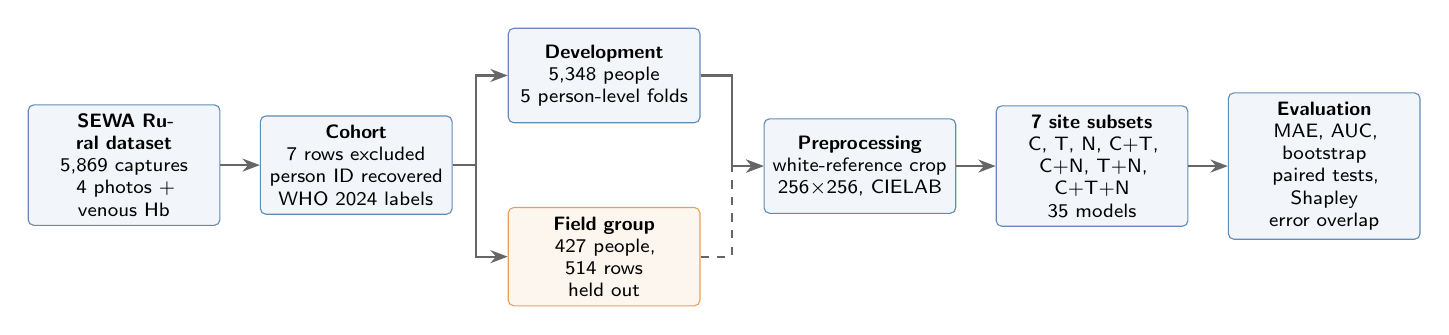
\begin{tikzpicture}[
  node distance=4mm and 5mm,
  box/.style={draw=c1!70,fill=c1!6,rounded corners=2pt,align=center,font=\sffamily\scriptsize,minimum height=12mm,text width=22mm},
  hl/.style={box,draw=c2!80,fill=c2!8},
  arr/.style={-{Stealth[length=2.2mm]},thick,draw=black!60}]
\node[box] (data) {\textbf{SEWA Rural dataset}\\5,869 captures\\4 photos + venous Hb};
\node[box,right=of data] (clean) {\textbf{Cohort}\\7 rows excluded\\person ID recovered\\WHO 2024 labels};
\node[box,above right=-1mm and 7mm of clean] (dev) {\textbf{Development}\\5,348 people\\5 person-level folds};
\node[hl,below right=-1mm and 7mm of clean] (field) {\textbf{Field group}\\427 people, 514 rows\\held out};
\node[box,right=8mm of $(dev.east)!0.5!(field.east)$] (prep) {\textbf{Preprocessing}\\white-reference crop\\256$\times$256, CIELAB};
\node[box,right=of prep] (models) {\textbf{7 site subsets}\\C, T, N, C+T,\\C+N, T+N, C+T+N\\35 models};
\node[box,right=of models] (eval) {\textbf{Evaluation}\\MAE, AUC, bootstrap\\paired tests, Shapley\\error overlap};
\draw[arr] (data) -- (clean);
\draw[arr] (clean.east) -- ++(3mm,0) |- (dev.west);
\draw[arr] (clean.east) -- ++(3mm,0) |- (field.west);
\draw[arr] (dev.east) -- ++(4mm,0) |- (prep.west);
\draw[arr,dashed] (field.east) -- ++(4mm,0) |- (prep.west);
\draw[arr] (prep) -- (models);
\draw[arr] (models) -- (eval);
\end{tikzpicture}
\caption{Study pipeline. The field group (orange) is predicted by every model but never used for training or model selection. C conjunctiva, T tongue, N nail beds.}
\label{fig:pipeline}
\end{figure*}

\subsection{Image preprocessing}
Following the base study, each photograph was cropped relative to the white paper reference, on the whole \cite{desai2026}, and if no reference was found, a centre square was employed. We located the paper as the largest bright, near-neutral region (CIELAB $L^*>150$; morphological opening, 15\,px kernel; at least 5\% of the image), rotated the image so the paper lay on top, and took the largest centred square directly below its edge, to a significant degree. Crops were, put simply, resized to $256\times256$ by area interpolation and converted to CIELAB. The same conjunctiva-oriented recipe was applied to every site. It found its target in 97.3\% of conjunctiva images but only 24.8\% of tongue, 36.6\% of nails-open and 49.4\% of nails-closed images, a shortcoming we return to in the Discussion.

\subsection{Model and training}
Each site has its own convolutional encoder (Fig.~\ref{fig:model}): a $7\times7$ stride-2 stem with 64 filters and max pooling, followed by two residual stages \cite{he2016} of one bottleneck block each (output 256 and 512 channels) and global average pooling to 512 features, broadly speaking. Indeed, one encoder is shared by the two nail views. Every model, including single-site models, receives the same metadata, so differences between models reflect the images alone, on the whole. Indeed, image features are concatenated with five metadata values (age/100, one-hot sex, pregnancy) and passed to a 256-unit hidden layer that outputs Hb relative to the training mean.

Models were trained from scratch with Adam \cite{kingma2015} (learning rate $10^{-4}$, exponential decay 0.97 per epoch), batch 32, 150 epochs, mixed precision, and random horizontal flips, on the whole. The epoch with the lowest validation MAE was kept. In turn, the conjunctiva model has 596,801 parameters, broadly speaking. What's more, one constant bias correction, the mean validation residual, was added to all predictions \cite{desai2026}. The loss was Huber ($\delta=1$) \cite{huber1964}, weighted per sample by the inverse square root of the frequency of its 1\gdl{} Hb bin \cite{yang2021}, to protect the rare severe cases. Think of it like this: the 35 models were trained with PyTorch \cite{paszke2019} on one RTX 3050 laptop GPU (about 19 minutes per conjunctiva model, 25 hours in total), in actual application.

\begin{figure}[t]
\centering
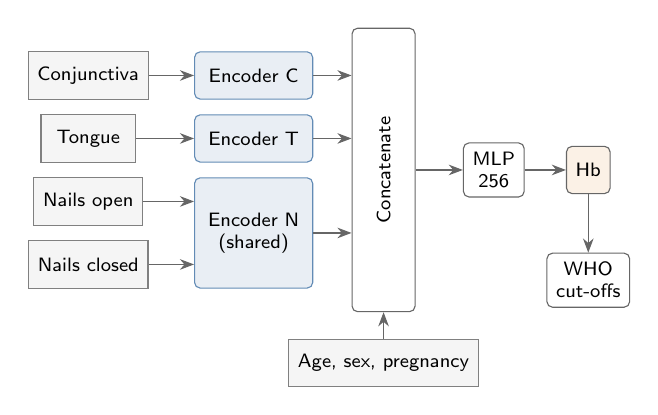
\begin{tikzpicture}[
  font=\sffamily\scriptsize,
  img/.style={draw=black!50,fill=black!4,minimum width=12mm,minimum height=6mm,align=center},
  enc/.style={draw=c1!70,fill=c1!10,rounded corners=2pt,minimum width=15mm,minimum height=6mm,align=center},
  op/.style={draw=black!60,fill=white,rounded corners=2pt,align=center,minimum height=6mm},
  arr/.style={-{Stealth[length=1.8mm]},draw=black!60}]
\node[img] (ic) at (0,1.6) {Conjunctiva};
\node[img] (it) at (0,0.8) {Tongue};
\node[img] (io) at (0,0)   {Nails open};
\node[img] (ix) at (0,-0.8){Nails closed};
\node[enc] (ec) at (2.1,1.6) {Encoder C};
\node[enc] (et) at (2.1,0.8) {Encoder T};
\node[enc,minimum height=14mm] (en) at (2.1,-0.4) {Encoder N\\(shared)};
\node[op,minimum height=36mm,minimum width=8mm] (cat) at (3.75,0.4) {\rotatebox{90}{Concatenate}};
\node[img] (meta) at (3.75,-2.05) {Age, sex, pregnancy};
\node[op] (mlp) at (5.15,0.4) {MLP\\256};
\node[op,fill=c2!12] (hb) at (6.35,0.4) {Hb};
\node[op] (who) at (6.35,-1.0) {WHO\\cut-offs};
\foreach \a/\b in {ic/ec,it/et} \draw[arr] (\a) -- (\b);
\draw[arr] (io.east) -- (en.west|-io.east);
\draw[arr] (ix.east) -- (en.west|-ix.east);
\draw[arr] (ec.east) -- (cat.west|-ec.east);
\draw[arr] (et.east) -- (cat.west|-et.east);
\draw[arr] (en.east) -- (cat.west|-en.east);
\draw[arr] (meta) -- (cat);
\draw[arr] (cat) -- (mlp);
\draw[arr] (mlp) -- (hb);
\draw[arr] (hb) -- (who);
\end{tikzpicture}
\caption{Model for C+T+N. Single- and two-site models keep only the matching encoders; all models receive the same metadata.}
\label{fig:model}
\end{figure}

\subsection{Baselines and references}
HemoCue venous and capillary readings and clinical examination were evaluated on the same rows, broadly speaking. To test whether a site carries Hb information beyond demographics, a no-image baseline was trained on age and sex, alongside pregnancy alone, employing histogram gradient boosting (depth 3, 200 iterations, learning rate 0.05) and linear regression \cite{pedregosa2011} on the same folds, broadly speaking.

\subsection{Statistical assessment}
Hb agreement was summarised by MAE, the share within $\pm1$\gdl, bias and Bland--Altman 95\% limits of agreement \cite{blandaltman1986}, in actual application. Indeed, the contribution of each site $i$ to performance $v$ (negative MAE, or AUC) was measured by its Shapley value \cite{shapley1953},
\begin{equation}
\phi_i=\sum_{K\subseteq S\setminus\{i\}}\frac{|K|!\,(|S|-|K|-1)!}{|S|!}\big[v(K\cup\{i\})-v(K)\big],
\end{equation}
where the empty set corresponds to the MAE of predicting the mean Hb, or an AUC of 0.5, broadly speaking. Three comparisons were fixed before analysis (C+T, C+N and C+T+N against C) and Holm-corrected as a family \cite{holm1979}; all others are exploratory. Indeed, paired model differences were computed on the same rows: MAE differences were tested with a $z$-test on per-person differences, and AUC differences with the paired DeLong test \cite{delong1988}. Error overlap compared the share of people misclassified by both of two single-site models with the share expected if their errors were independent. Confidence intervals are percentile bootstraps over people, with 1,000 resamples \cite{efron1979}. Classification used the AUC of the ranking score for each task and sensitivity at fixed specificity. Indeed, subgroups with at least 30 rows were analysed by age, pregnancy, sex, severity band, phone, and light. Reporting follows STARD 2015 and TRIPOD+AI where applicable \cite{bossuyt2015,collins2024}.

% =====================================================================
\section{Results}

\subsection{Overall performance (RQ1)}
On development data, every model including the conjunctiva hit an MAE of 1.18--1.20\gdl{} and an any-anemia AUC of 0.763--0.768, with severe-anemia AUCs of 0.93--0.94, on the whole (Table~\ref{tab:overall}, Fig.~\ref{fig:mae}). Indeed, the no-image baseline got 1.63\gdl{} (linear regression 1.68\gdl) and an AUC of 0.63, against 1.71\gdl{} for always predicting the mean, in real-world scenarios. Across the five folds, the conjunctiva model's MAE ranged from 1.18 to 1.26\gdl. So, models without the conjunctiva were clearly worse, like nails 1.42\gdl{} and tongue 1.61\gdl.

\begin{table*}[t]
\centering\small
\caption{Hb estimation and anemia classification for every site combination. Development: pooled out-of-fold predictions (5,348 people). Field: average of the five fold models (427 people). 95\% bootstrap CIs in brackets. Best image model per column in bold.}
\label{tab:overall}
\setlength{\tabcolsep}{4.2pt}
\begin{adjustbox}{max width=\textwidth}
\begin{tabular}{@{}l ccccc @{\hskip 10pt} cccc@{}}
\toprule
 & \multicolumn{5}{c}{Development (cross-validated)} & \multicolumn{4}{c}{Field group} \\
\cmidrule(lr){2-6}\cmidrule(l){7-10}
Input & MAE (g/dL) & $\pm$1 g/dL & AUC any & AUC mod/sev & AUC severe & MAE (g/dL) & Bias & AUC any & AUC severe \\
\midrule
C       & 1.203 [1.18, 1.23] & 0.52 & 0.765 [0.75, 0.78] & 0.803 & 0.928 & 1.216 [1.13, 1.31] & $-$0.28 & 0.722 & 0.932 \\
C+T     & 1.197 [1.17, 1.23] & 0.52 & 0.763 [0.75, 0.78] & 0.805 & 0.930 & \textbf{1.196} [1.12, 1.28] & $-$0.46 & 0.742 & 0.949 \\
C+N     & \textbf{1.176} [1.15, 1.20] & \textbf{0.53} & 0.764 [0.75, 0.78] & \textbf{0.810} & \textbf{0.937} & 1.288 [1.20, 1.38] & $-$0.53 & 0.740 & 0.943 \\
C+T+N   & 1.178 [1.15, 1.21] & 0.52 & \textbf{0.768} [0.75, 0.78] & 0.807 & 0.936 & 1.269 [1.19, 1.36] & $-$0.58 & \textbf{0.757} & \textbf{0.963} \\
N       & 1.415 [1.38, 1.45] & 0.45 & 0.707 [0.69, 0.72] & 0.745 & 0.876 & 2.309 [2.15, 2.47] & $-$1.96 & 0.734 & 0.913 \\
T+N     & 1.395 [1.37, 1.43] & 0.46 & 0.710 [0.69, 0.72] & 0.747 & 0.879 & 2.131 [1.98, 2.27] & $-$1.74 & 0.725 & 0.890 \\
T       & 1.605 [1.57, 1.64] & 0.41 & 0.654 [0.64, 0.67] & 0.681 & 0.767 & 1.606 [1.48, 1.72] & $-$0.77 & 0.642 & 0.791 \\
\midrule
No image (metadata only) & 1.629 & -- & 0.634 & 0.669 & 0.728 & 1.661 & $-$0.70 & 0.627 & 0.698 \\
Predict the mean Hb & 1.705 & -- & 0.500 & 0.500 & 0.500 & 1.415 & -- & 0.500 & 0.500 \\
HemoCue, venous & 0.473 & -- & 0.983 & 0.992 & 0.998 & 0.384 & $+$0.34 & 0.992 & 0.999 \\
HemoCue, capillary$^{a}$ & 0.499 & -- & 0.942 & 0.963 & 0.997 & 0.452 & $+$0.07 & 0.963 & 0.998 \\
\bottomrule
\end{tabular}
\end{adjustbox}
\par\vspace{2pt}\raggedright\footnotesize $^{a}$Development capillary readings were available for 3,586 rows. The field group contains 29 people with severe anemia, so field severe AUCs are imprecise.
\end{table*}

\begin{figure}[t]
\centering
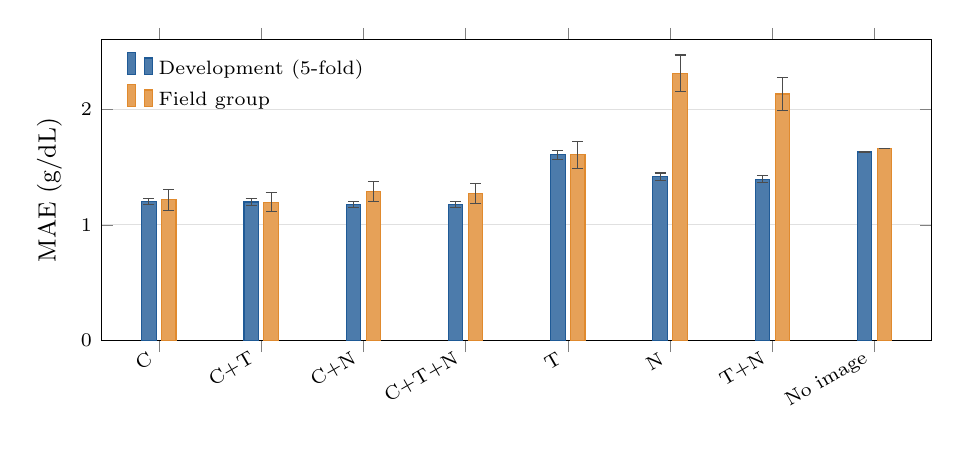
\begin{tikzpicture}
\begin{axis}[
  width=\columnwidth, height=5.4cm,
  ybar, bar width=5.2pt,
  ymin=0, ymax=2.6,
  ylabel={MAE (g/dL)}, ylabel style={font=\small},
  symbolic x coords={C,C+T,C+N,C+T+N,T,N,T+N,Meta},
  xtick=data, xticklabels={C,C+T,C+N,C+T+N,T,N,T+N,No image},
  x tick label style={font=\scriptsize,rotate=30,anchor=east},
  y tick label style={font=\scriptsize},
  legend style={font=\scriptsize,at={(0.02,0.98)},anchor=north west,draw=none,fill=none},
  legend cell align=left,
  enlarge x limits=0.08,
  ymajorgrids, grid style={black!12},
  error bars/y dir=both, error bars/y explicit,
  error bars/error bar style={black!70},
]
\addplot[fill=c1!80,draw=c1] coordinates {
 (C,1.203) +- (0,0.028) (C+T,1.197) +- (0,0.027) (C+N,1.176) +- (0,0.025)
 (C+T+N,1.178) +- (0,0.026) (T,1.605) +- (0,0.037) (N,1.415) +- (0,0.033)
 (T+N,1.395) +- (0,0.031) (Meta,1.629) +- (0,0)};
\addplot[fill=c2!80,draw=c2] coordinates {
 (C,1.216) +- (0,0.091) (C+T,1.196) +- (0,0.081) (C+N,1.288) +- (0,0.090)
 (C+T+N,1.269) +- (0,0.086) (T,1.606) +- (0,0.117) (N,2.309) +- (0,0.159)
 (T+N,2.131) +- (0,0.141) (Meta,1.661) +- (0,0)};
\legend{Development (5-fold), Field group}
\end{axis}
\end{tikzpicture}
\caption{MAE by input with 95\% CIs (error bars show the average half-width). Conjunctiva models are stable across settings; nail models degrade sharply in the field group.}
\label{fig:mae}
\end{figure}

\subsection{Does adding a site help? (RQ1)}
On development data, adding nails lowered MAE by 0.027\gdl{} (95\% CI 0.007--0.045; Holm $p=0.020$) and adding both tongue and nails by 0.025\gdl{} (Holm $p=0.047$), in actual application (Table~\ref{tab:paired}). In the field group the direction reversed, namely C+N was 0.072\gdl{} \emph{worse} than C (unadjusted $p=0.043$; Holm $p=0.13$), and no combination improved MAE after correction, to a significant degree. The only field gain was a 0.035 higher any-anemia AUC for C+T+N (unadjusted DeLong $p=0.027$), which doesn't survive correction for three tests. Adding the tongue alone gave no detectable change on development data, and none of these gains appeared in any-anemia AUC.

\begin{table}[t]
\centering\small
\caption{Pre-specified paired comparisons against the conjunctiva (C). Negative $\Delta$MAE favours the larger model. $p_\mathrm{H}$: Holm-corrected; $p_\mathrm{D}$: unadjusted DeLong for any-anemia AUC.}
\label{tab:paired}
\setlength{\tabcolsep}{3pt}
\begin{tabularx}{\columnwidth}{@{}lXccc@{}}
\toprule
Model & $\Delta$MAE [95\% CI] & $p_\mathrm{H}$ & $\Delta$AUC & $p_\mathrm{D}$ \\
\midrule
\multicolumn{5}{@{}l}{\emph{Development (n = 5,348)}}\\
C+T   & $-0.006$ [$-0.024$, 0.014] & 0.51 & $-0.002$ & 0.70 \\
C+N   & $-0.027$ [$-0.045$, $-0.007$] & \textbf{0.020} & $-0.001$ & 0.78 \\
C+T+N & $-0.025$ [$-0.046$, $-0.002$] & \textbf{0.047} & $+0.003$ & 0.64 \\
\midrule
\multicolumn{5}{@{}l}{\emph{Field group (n = 427)}}\\
C+T   & $-0.020$ [$-0.091$, 0.037] & 0.52 & $+0.020$ & 0.12 \\
C+N   & $+0.072$ [0.005, 0.138] & 0.13 & $+0.017$ & 0.23 \\
C+T+N & $+0.054$ [$-0.020$, 0.124] & 0.33 & $+0.035$ & 0.027 \\
\bottomrule
\end{tabularx}
\end{table}

\subsection{Why the extra sites add little (RQ2)}

\subsubsection{The tongue is usually close to uninformative}
The tongue model's MAE (1.605\gdl) and AUC (0.654) barely improve on the no-image baseline (1.629\gdl, 0.634), in many respects. As well, in the field group the two are, in practice, indistinguishable (1.606 vs 1.661\gdl; AUC 0.642 vs 0.627), in many respects. Its Shapley contribution to MAE was 0.04\gdl{} on development data and $-0.02$\gdl{} in the field group (Fig.~\ref{fig:shapley}).

\subsubsection{The nails carry signal but are redundant and fragile}
Nail images clearly beat the no-image baseline (1.415 vs 1.629\gdl), and in the field group their AUC (0.734) matched that of the conjunctiva (0.722), in many respects. Their mistakes, though, happened together with the conjunctiva's: both models misclassified any anemia in 13.7\% of people, against 7.0\% expected under independence, in actual application (Table~\ref{tab:overlap}). In the field group, nail models under-estimated Hb by 1.96\gdl{} on average, and every one of the five fold models did so ($-1.56$ to $-2.58$\gdl). As well, their mean prediction fell from 10.06\gdl{} (development) to 8.69\gdl{} (field). Part of this shift is common to all models, because field participants were less anemic (mean Hb 10.45 vs 10.05\gdl; 60\% vs 73\% anemic), and the no-image baseline was itself biased by $-0.70$\gdl. The remaining $\approx1.3$\gdl{} or so is specific to the nail images. The bias grew with ambient light, from $-1.30$\gdl{} below 100\,lux to $-2.53$\gdl{} above 1,500\,lux, but was already large in dim light. That said, lighting explains it only in part. As a result, the nails' Shapley contribution to MAE turned from $+0.14$\gdl{} on development data to $-0.42$\gdl{} in the field. Meanwhile, their contribution to AUC stayed positive.

\begin{table}[t]
\centering\small
\caption{Error overlap for any anemia: share of people misclassified by both single-site models, against the share expected if errors were independent.}
\label{tab:overlap}
\begin{tabularx}{\columnwidth}{@{}Xcccc@{}}
\toprule
 & \multicolumn{2}{c}{Development} & \multicolumn{2}{c}{Field} \\
\cmidrule(lr){2-3}\cmidrule(l){4-5}
Pair & Both wrong & Expected & Both wrong & Expected \\
\midrule
C and T & 15.6\% & 7.3\% & 20.1\% & 12.4\% \\
C and N & 13.7\% & 7.0\% & 19.9\% & 12.0\% \\
N and T & 17.0\% & 7.9\% & 28.8\% & 13.3\% \\
\bottomrule
\end{tabularx}
\end{table}

\begin{figure}[t]
\centering
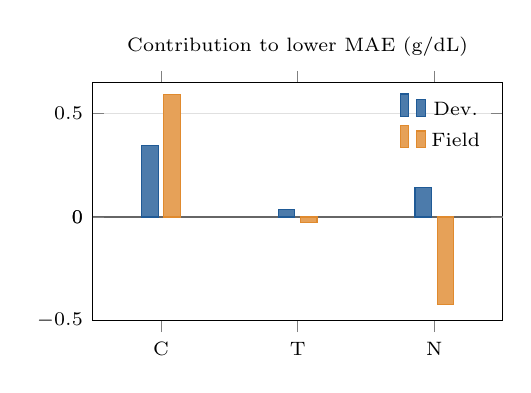
\begin{tikzpicture}
\begin{axis}[
  width=0.56\columnwidth, height=4.6cm,
  ybar, bar width=6pt, ymin=-0.5, ymax=0.65,
  symbolic x coords={C,T,N}, xtick=data,
  title={\scriptsize Contribution to lower MAE (g/dL)},
  x tick label style={font=\scriptsize}, y tick label style={font=\scriptsize},
  enlarge x limits=0.25, ymajorgrids, grid style={black!12},
  extra y ticks={0}, extra y tick style={grid style={black!60}},
  legend style={font=\scriptsize,at={(0.98,0.98)},anchor=north east,draw=none,fill=none}]
\addplot[fill=c1!80,draw=c1] coordinates {(C,0.347) (T,0.037) (N,0.143)};
\addplot[fill=c2!80,draw=c2] coordinates {(C,0.592) (T,-0.025) (N,-0.422)};
\legend{Dev.,Field}
\end{axis}
\end{tikzpicture}\hfill
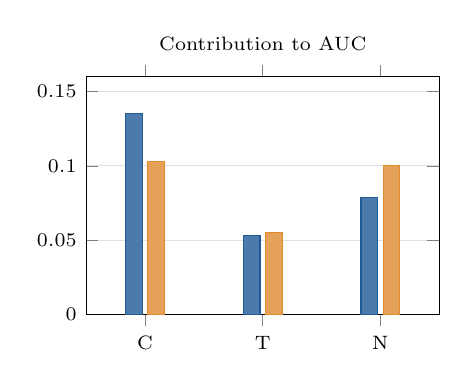
\begin{tikzpicture}
\begin{axis}[
  width=0.50\columnwidth, height=4.6cm,
  ybar, bar width=6pt, ymin=0, ymax=0.16,
  symbolic x coords={C,T,N}, xtick=data,
  title={\scriptsize Contribution to AUC},
  x tick label style={font=\scriptsize}, y tick label style={font=\scriptsize,/pgf/number format/fixed},
  scaled y ticks=false,
  enlarge x limits=0.25, ymajorgrids, grid style={black!12}]
\addplot[fill=c1!80,draw=c1] coordinates {(C,0.135) (T,0.053) (N,0.079)};
\addplot[fill=c2!80,draw=c2] coordinates {(C,0.103) (T,0.055) (N,0.100)};
\end{axis}
\end{tikzpicture}
\caption{Shapley contribution of each site. Nails help ranking (AUC) in both settings but harm calibration (MAE) in the field group.}
\label{fig:shapley}
\end{figure}

\subsubsection{Regression toward the mean}
All models compress predictions toward the middle of the Hb range (Fig.~\ref{fig:bias}). For the conjunctiva model, Hb was under-estimated in people with normal Hb ($-1.05$\gdl) and over-estimated in severe anemia ($+1.15$\gdl), the most clinically significant direction. MAE by band was 1.26, 0.89, 1.22 and 1.61\gdl{} for normal, mild, moderate and severe anemia, respectively. The tongue model's severe-anemia bias hit $+3.14$\gdl.

\begin{figure}[t]
\centering
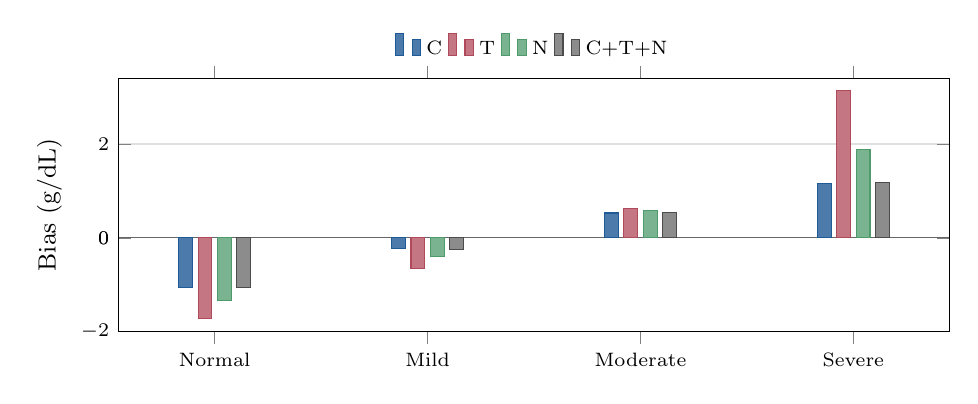
\begin{tikzpicture}
\begin{axis}[
  width=\columnwidth, height=4.8cm,
  ybar, bar width=5pt, ymin=-2, ymax=3.4,
  ylabel={Bias (g/dL)}, ylabel style={font=\small},
  symbolic x coords={Normal,Mild,Moderate,Severe}, xtick=data,
  x tick label style={font=\scriptsize}, y tick label style={font=\scriptsize},
  enlarge x limits=0.15, ymajorgrids, grid style={black!12},
  extra y ticks={0}, extra y tick style={grid style={black!60}},
  legend style={font=\scriptsize,at={(0.5,1.03)},anchor=south,draw=none,fill=none},
  legend columns=4]
\addplot[fill=c1!80,draw=c1] coordinates {(Normal,-1.05) (Mild,-0.23) (Moderate,0.53) (Severe,1.15)};
\addplot[fill=c4!75,draw=c4] coordinates {(Normal,-1.72) (Mild,-0.66) (Moderate,0.62) (Severe,3.14)};
\addplot[fill=c3!75,draw=c3] coordinates {(Normal,-1.34) (Mild,-0.39) (Moderate,0.59) (Severe,1.89)};
\addplot[fill=black!45,draw=black!70] coordinates {(Normal,-1.05) (Mild,-0.24) (Moderate,0.54) (Severe,1.18)};
\legend{C, T, N, C+T+N}
\end{axis}
\end{tikzpicture}
\caption{Mean prediction error by WHO severity band (development). Positive values mean Hb is over-estimated, so anemia is under-called.}
\label{fig:bias}
\end{figure}

\begin{table*}[!t]
\centering\small
\caption{Comparison with published smartphone-based Hb estimation systems. Values are as reported by each study; cohorts, cut-offs and validation designs differ.}
\label{tab:literature}
\setlength{\tabcolsep}{4pt}
\renewcommand{\arraystretch}{1.15}
\newcolumntype{L}{>{\raggedright\arraybackslash}X}
\begin{tabularx}{\textwidth}{@{}>{\raggedright\arraybackslash}p{2.3cm}>{\raggedright\arraybackslash}p{2.2cm}LLcccL@{}}
\toprule
Study & Site(s) & Method & Population and validation & MAE (g/dL) & 95\% LoA (g/dL) & AUC any & Other \\
\midrule
Mannino et al.\ 2018 \cite{mannino2018} & Fingernail & Colour + image metadata, multilinear regression & 337 US patients and controls, iPhone 5s; 100 validation & 0.97 & $\pm$2.4 & 0.88$^{a}$ & Sens.\ 92\%, spec.\ 76\% at $<$11\gdl \\
Zhao et al.\ 2024 \cite{zhao2024} & Conjunctiva & Hue-ratio algorithm (RAW images) & 435 US emergency patients, one phone & -- & $-$4.73 to 4.93 & 0.76 & Accuracy 75.4\%; AUC 0.92 at $<$7\gdl \\
Lin et al.\ 2025 \cite{lin2025} & Conjunctiva, palm, fingernail (one at a time) & ResNet-50 + attention, body-part tag, dual loss & EYES-DEFY (218), 5-fold; NTUH emergency (101), 4-fold & 1.21 / 2.02 & -- & -- & Accuracy 0.85 / 0.72; F1 0.83 / 0.79 \\
Desai et al.\ 2026 \cite{desai2026} & Conjunctiva (+T, N ablation) & 2-stage ResNet + metadata & Rural India, 3 phones; one 70:15:15 split, 777 test & 1.12 & $-$2.90 to 2.85 & 0.80 & Severe AUC 0.93; sens./spec.\ 70/70\% \\
\midrule
\textbf{This study}, C & Conjunctiva & 2-stage bottleneck ResNet + metadata & Same population; 5-fold by person (5,348); field group (427) & 1.20 & $\pm$3.07 & 0.77 & Severe AUC 0.93; sens.\ 69\% at 70\% spec. \\
\textbf{This study}, C+T+N & All three & Per-site encoders, late concatenation & As above & 1.18 & $\pm$2.96 & 0.77 & Severe AUC 0.94; field MAE 1.27 \\
\bottomrule
\end{tabularx}
\par\vspace{2pt}\raggedright\footnotesize $^{a}$At a cut-off of 11\gdl. LoA: Bland--Altman 95\% limits of agreement. BPANet values are for the retrospective / prospective datasets.
\end{table*}

\subsection{Clinical comparison and subgroups (RQ3)}
At the clinicians' own specificity, the conjunctiva model detected 80\% of anemia on development data (clinicians 74\%), and 37--44\% in the field group, where clinicians detected only 27\% at 91\% specificity, broadly speaking (Table~\ref{tab:clinic}). Indeed, thresholding predicted Hb directly at each person's cut-off, though, gave 88\% sensitivity at only 40\% specificity, so a deployment threshold must be chosen deliberately, in many respects. At the base study's operating points, the conjunctiva model detected 69\% of anemia at 70\% specificity and 88\% of severe anemia at 80\% specificity (C+T+N: 68\% and 91\%).

\begin{table}[t]
\centering\small
\caption{Any-anemia detection: models at the specificity achieved by clinical examination, and HemoCue AUC.}
\label{tab:clinic}
\setlength{\tabcolsep}{4pt}
\begin{tabularx}{\columnwidth}{@{}Xcc@{}}
\toprule
 & Development & Field \\
\midrule
Clinician sensitivity / specificity & 73.8 / 53.3\% & 26.5 / 90.6\% \\
C, sensitivity at clinician specificity & 80.4\% & 44.4\%$^{a}$ \\
C+T, sensitivity at clinician specificity & 80.1\% & 37.4\% \\
C+T+N, sensitivity at clinician specificity & 82.0\% & 41.2\% \\
HemoCue venous AUC & 0.983 & 0.992 \\
\bottomrule
\multicolumn{3}{@{}l}{\footnotesize $^{a}$All 514 field conjunctiva captures; other field rows $n=427$.}
\end{tabularx}
\end{table}

Across phones and light levels, performance was, in effect, broadly stable (Table~\ref{tab:subgroups}). Indeed, pregnant women had the lowest error but also the lowest AUC (0.69), consistent with Hb values clustered near their lower cut-off of 11\gdl. Men had the highest error but the highest AUC (0.82--0.84), in many respects. Captures flagged for nail polish or henna didn't do worse.

\begin{table}[t]
\centering\small
\caption{Development subgroups: MAE (g/dL) and any-anemia AUC.}
\label{tab:subgroups}
\setlength{\tabcolsep}{3.5pt}
\begin{tabularx}{\columnwidth}{@{}Xrcccc@{}}
\toprule
 & & \multicolumn{2}{c}{C} & \multicolumn{2}{c}{C+T+N} \\
\cmidrule(lr){3-4}\cmidrule(l){5-6}
Subgroup & $n$ & MAE & AUC & MAE & AUC \\
\midrule
Age $<$15 & 772 & 1.22 & 0.739 & 1.15 & 0.731 \\
Age $\ge$15 & 4,576 & 1.20 & 0.765 & 1.18 & 0.768 \\
Pregnant & 2,601 & 1.12 & 0.693 & 1.13 & 0.690 \\
Non-pregnant women & 1,457 & 1.28 & 0.808 & 1.22 & 0.808 \\
Men & 514 & 1.39 & 0.816 & 1.34 & 0.841 \\
Samsung A05 & 1,995 & 1.16 & 0.764 & 1.16 & 0.760 \\
Samsung A14 & 1,577 & 1.28 & 0.766 & 1.19 & 0.775 \\
Samsung S24 & 1,776 & 1.19 & 0.766 & 1.19 & 0.771 \\
Lowest light tertile & 1,755 & 1.18 & 0.758 & 1.15 & 0.762 \\
Highest light tertile & 1,796 & 1.21 & 0.777 & 1.21 & 0.771 \\
Polish or henna noted & 319 & 1.03 & 0.816 & 1.05 & 0.799 \\
\bottomrule
\end{tabularx}
\end{table}

\subsection{Comparison with published systems}
On the same population, the base study's conjunctiva model reported a lower MAE (1.12 vs 1.20\gdl) and higher any-anemia AUC (0.80 vs 0.77) on its single test split, with near-identical severe-anemia AUC (0.93) and near-identical sensitivity at its operating points, on the whole \cite{desai2026} (Table~\ref{tab:literature}, Fig.~\ref{fig:literature}). Our limits of agreement ($\pm3.07$\gdl) are narrower than those of Zhao et al.\ ($-4.73$ to 4.93\gdl) \cite{zhao2024}, to a significant degree. Our development MAE is, indeed, close to BPANet's curated eye-dataset result while being far lower than its prospective emergency-department MAE of 2.02\gdl{} \cite{lin2025}. Mannino et al.\ reported the lowest error (MAE 0.97\gdl) in 100 validation subjects, under uniform lighting with one phone and manually chosen nail regions \cite{mannino2018}. As the cohorts, Hb ranges and validation designs differ, these figures show context rather than a ranking.

\begin{figure}[t]
\centering
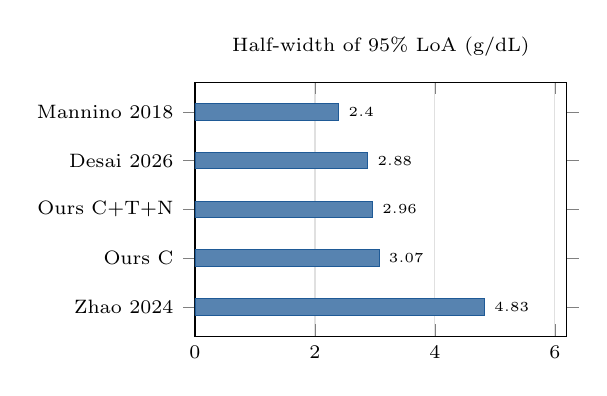
\begin{tikzpicture}
\begin{axis}[
  width=0.52\columnwidth, height=4.8cm,
  xbar, bar width=6pt, xmin=0, xmax=6.2,
  title={\scriptsize Half-width of 95\% LoA (g/dL)},
  symbolic y coords={Zhao 2024,Ours C,Ours C+T+N,Desai 2026,Mannino 2018},
  ytick=data, y tick label style={font=\scriptsize},
  x tick label style={font=\scriptsize},
  enlarge y limits=0.15, xmajorgrids, grid style={black!12},
  nodes near coords, nodes near coords style={font=\tiny},
  every node near coord/.append style={/pgf/number format/fixed,/pgf/number format/precision=2}]
\addplot[fill=c1!75,draw=c1] coordinates {(4.83,Zhao 2024) (3.07,Ours C) (2.96,Ours C+T+N) (2.88,Desai 2026) (2.40,Mannino 2018)};
\end{axis}
\end{tikzpicture}\hfill
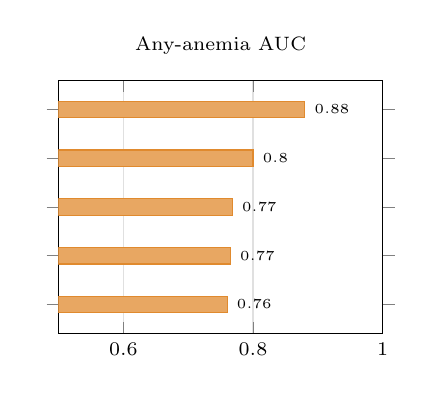
\begin{tikzpicture}
\begin{axis}[
  width=0.47\columnwidth, height=4.8cm,
  xbar, bar width=6pt, xmin=0.5, xmax=1.0,
  title={\scriptsize Any-anemia AUC},
  symbolic y coords={Zhao 2024,Ours C,Ours C+T+N,Desai 2026,Mannino 2018},
  ytick=data, yticklabels={,,,,},
  x tick label style={font=\scriptsize,/pgf/number format/fixed},
  enlarge y limits=0.15, xmajorgrids, grid style={black!12},
  nodes near coords, nodes near coords style={font=\tiny},
  every node near coord/.append style={/pgf/number format/fixed,/pgf/number format/precision=2}]
\addplot[fill=c2!75,draw=c2] coordinates {(0.76,Zhao 2024) (0.765,Ours C) (0.768,Ours C+T+N) (0.80,Desai 2026) (0.88,Mannino 2018)};
\end{axis}
\end{tikzpicture}
\caption{Agreement and discrimination reported by published systems (rows aligned). Mannino's AUC uses an 11\gdl{} cut-off; cohorts differ, so bars give context, not a ranking.}
\label{fig:literature}
\end{figure}

% =====================================================================
\section{Discussion}

\subsection{Principal findings}
Adding the nail beds made a small but statistically significant gain on development data that didn't transfer to field conditions, and adding the tongue created no gain at all. These findings validate the base study's conclusion \cite{desai2026}, now with uncertainty estimates, paired tests and an explanation of each failure, in actual application. Across seven site combinations, five folds and an independent field group, the conjunctiva carried most of the usable Hb information, in many respects.

\subsection{Why extra sites fail}
The three sites fail for distinct reasons. The tongue is \emph{uninformative} under our pipeline: it performs at the level of a model that sees no image, broadly speaking. The nail beds are \emph{redundant}: their errors fall on the same people as the conjunctiva's, so concatenating their features adds little that the conjunctiva hadn't already captured. They are also \emph{fragile}: a stable ranking signal (field AUC 0.73) sat on a shifted baseline, so their absolute Hb estimates were biased by about 2\gdl{} in a new setting. This combination, a development-set gain with a field-set loss, is the most essential applied lesson: improvements from adding modalities should be verified on independent data before rollout, in real-world scenarios.

\subsection{Comparison with prior work}
Our conjunctiva results are close to those of the base study on the same population (MAE 1.20 vs 1.12\gdl; severe AUC 0.93 in both), in real-world scenarios. The gap is plausibly explained by the base study's removal of 279 captures with incomplete data or crop errors, by architectural differences from its released code \cite{googlecode}, and by our check over all 5,348 development people rather than one 777-person split, to a significant degree. Mannino et al.\ showed that fingernail colour can, in practice, track Hb closely in a controlled setting \cite{mannino2018}. Our nail models were far weaker and less stable, which points to acquisition and preprocessing rather than an absence of signal. BPANet ranked fingernails as its weakest site and also lost accuracy between retrospective and prospective data \cite{lin2025}, in line with our findings.

\subsection{Clinical implications}
At matched specificity the conjunctiva model detected more anemia than clinical examination in both settings, supporting its use as a triage aid where blood testing is unavailable. It doesn't approach HemoCue (MAE 0.38--0.50\gdl), and it over-estimates Hb in severe anemia by about 1.2\gdl, broadly speaking. Any rollout therefore needs a deliberately chosen, conservative threshold, rather than the raw WHO cut-off, which flagged 60\% of non-anemic people, on the whole.

\subsection{Limitations}
For starters, one conjunctiva-oriented crop was employed for every site. It located the tongue and nails in only 25--49\% of images. Part of their weakness may reflect cropping rather than physiology, and a site-specific preprocessing pipeline is the next step. Second, the data come from one hospital with sampling enriched for severe anemia, which can inflate diagnostic accuracy \cite{rutjes2006}. Third, our network differs from the base study's released architecture, and each model was trained with a single seed. Fourth, field estimates average five models, whereas development estimates come from single models; individual conjunctiva models reached field MAEs of 1.30--1.36\gdl. Fifth, the field group includes only 29 people with severe anemia, and DeLong $p$ values aren't corrected for multiplicity. One last thing: settings were picked on validation data from fold 0 after its test scores had been inspected, and trimester was unavailable for pregnancy cut-offs.

\subsection{Future work}
Planned work includes site-specific crops for the tongue and nails, the base study's published architecture and pretrained backbones, alternative fusion strategies, light and colour normalisation for nail images, calibration of operating thresholds, and validation in community settings, in many respects.

% =====================================================================
\section{Conclusion}
A smartphone photograph of the conjunctiva can screen for anemia with accuracy that exceeds clinical examination and is stable across phones and settings, in many respects. Tongue images add nothing beyond age, sex and pregnancy, and nail images, although informative, overlap with the conjunctiva and become miscalibrated in field conditions, to a significant degree. For now, the conjunctiva alone is the most beneficial and solid site for smartphone-based anemia screening.

% =====================================================================
\section*{Declarations}
\small
\noindent\textbf{Data availability}\enspace The dataset is available from Hugging Face under gated access \cite{sewa2026}; its licence forbids redistribution, so no images are shared here. Derived result tables are available from the corresponding author.

\noindent\textbf{Code availability}\enspace [Repository link to be added.]

\noindent\textbf{Ethics}\enspace Secondary analysis of a de-identified public dataset under its data-use agreement. The original study was approved by the SEWA Rural Institutional Ethics Committee (CTRI/2023/07/055313) with written informed consent \cite{desai2026}.

\noindent\textbf{Funding}\enspace [To be completed.]

\noindent\textbf{Competing interests}\enspace The authors declare no competing interests.

\noindent\textbf{Author contributions}\enspace [To be completed.]

\noindent\textbf{Acknowledgements}\enspace We thank SEWA Rural and the study participants for making the dataset available.

% =====================================================================
\begin{thebibliography}{99}
\footnotesize
\setlength{\itemsep}{1pt}

\bibitem{gbd2023} GBD 2021 Anaemia Collaborators. Prevalence, years lived with disability, and trends in anaemia burden by severity and cause, 1990--2021: findings from the Global Burden of Disease Study 2021. Lancet Haematol. 2023;10(9):e713--e734. doi:10.1016/S2352-3026(23)00160-6

\bibitem{kinyoki2021} Kinyoki D, Osgood-Zimmerman AE, Bhattacharjee NV, et al. Anemia prevalence in women of reproductive age in low- and middle-income countries between 2000 and 2018. Nat Med. 2021;27(10):1761--1782. doi:10.1038/s41591-021-01498-0

\bibitem{nfhs5} International Institute for Population Sciences (IIPS). National Family Health Survey (NFHS-5), 2019--21: India. Mumbai: IIPS; 2021.

\bibitem{who2024} World Health Organization. Guideline on haemoglobin cutoffs to define anaemia in individuals and populations. Geneva: WHO; 2024.

\bibitem{chalco2005} Chalco JP, Huicho L, Alamo C, Carreazo NY, Bada CA. Accuracy of clinical pallor in the diagnosis of anaemia in children: a meta-analysis. BMC Pediatr. 2005;5:46. doi:10.1186/1471-2431-5-46

\bibitem{kalantri2010} Kalantri A, Karambelkar M, Joshi R, Kalantri S, Jajoo U. Accuracy and reliability of pallor for detecting anaemia: a hospital-based diagnostic accuracy study. PLoS One. 2010;5(1):e8545.

\bibitem{stoltzfus1999} Stoltzfus RJ, Edward-Raj A, Dreyfuss ML, et al. Clinical pallor is useful to detect severe anemia in populations where anemia is prevalent and severe. J Nutr. 1999;129(9):1675--1681.

\bibitem{collings2016} Collings S, Thompson O, Hirst E, Goossens L, George A, Weinkove R. Non-invasive detection of anaemia using digital photographs of the conjunctiva. PLoS One. 2016;11(4):e0153286. doi:10.1371/journal.pone.0153286

\bibitem{suner2021} Suner S, Rayner J, Ozturan IU, et al. Prediction of anemia and estimation of hemoglobin concentration using a smartphone camera. PLoS One. 2021;16(7):e0253495. doi:10.1371/journal.pone.0253495

\bibitem{zhao2024} Zhao L, Vidwans A, Bearnot CJ, Rayner J, Lin T, Baird J, Suner S, Jay GD. Prediction of anemia in real-time using a smartphone camera processing conjunctival images. PLoS One. 2024;19(5):e0302883. doi:10.1371/journal.pone.0302883

\bibitem{mannino2018} Mannino RG, Myers DR, Tyburski EA, et al. Smartphone app for non-invasive detection of anemia using only patient-sourced photos. Nat Commun. 2018;9:4924. doi:10.1038/s41467-018-07262-2

\bibitem{mannino2025} Mannino RG, Sullivan J, Frediani JK, et al. Real-world implementation of a noninvasive, AI-augmented, anemia-screening smartphone app and personalization for hemoglobin level self-monitoring. Proc Natl Acad Sci USA. 2025;122(20).

\bibitem{wang2016} Wang EJ, Li W, Hawkins D, Gernsheimer T, Norby-Slycord C, Patel SN. HemaApp: noninvasive blood screening of hemoglobin using smartphone cameras. In: Proc ACM UbiComp; 2016:593--604.

\bibitem{wang2017} Wang EJ, Li W, Zhu J, Rana R, Patel SN. Noninvasive hemoglobin measurement using unmodified smartphone camera and white flash. Annu Int Conf IEEE Eng Med Biol Soc. 2017;2017:2333--2336.

\bibitem{appiahene2023} Appiahene P, Asare JW, Donkoh ET, Dimauro G, Maglietta R. Detection of iron deficiency anemia by medical images: a comparative study of machine learning algorithms. BioData Min. 2023;16:2.

\bibitem{asare2023} Asare JW, Appiahene P, Donkoh ET, Dimauro G. Iron deficiency anemia detection using machine learning models: a comparative study of fingernails, palm and conjunctiva of the eye images. Eng Rep. 2023;e12667.

\bibitem{mahmud2023} Mahmud S, Donmez TB, Mansour M, Kutlu M, Freeman C. Anemia detection through non-invasive analysis of lip mucosa images. Front Big Data. 2023;6:1241899.

\bibitem{hasan2021} Hasan MK, Aziz MH, Zarif MII, et al. Noninvasive hemoglobin level prediction in a mobile phone environment: state of the art review and recommendations. JMIR Mhealth Uhealth. 2021;9(4):e16806. doi:10.2196/16806

\bibitem{mohamed2024} Mohamed M, Salama R, Ahmed M, Aboul-Yazeed RS. AI-powered noninvasive anemia detection: a review of image-based techniques. Adv Sci Technol J. 2024;1(2):1--30.

\bibitem{desai2026} Desai S, Gadgil S, Gottala VA, et al. Smartphone-based non-invasive classification of anemia severity using deep learning: a cross-sectional study in rural India. medRxiv [preprint]. 2026. doi:10.64898/2026.10.22.26366247

\bibitem{sewa2026} SEWA Rural. Anemia Detection---Multi-Modal Clinical SEWA Rural Dataset, v1.0 [dataset]. Hugging Face; 2026. \url{https://huggingface.co/datasets/sewa-rural-care/anemia-survey-dataset}

\bibitem{googlecode} Google Health. non-invasive-anemia-ai [source code]. GitHub; 2026. \url{https://github.com/Google-Health/google-health/tree/master/non-invasive-anemia-ai}

\bibitem{dimauro2023} Dimauro G, Griseta ME, Camporeale MG, Clemente F, Guarini A, Maglietta R. An intelligent non-invasive system for automated diagnosis of anemia exploiting a novel dataset. Artif Intell Med. 2023;136:102477.

\bibitem{hong2025} Hong S, Park SM, Kwon S, et al. Radiomic identification of anemia features in monochromatic conjunctiva photographs in school-age children. Biophotonics Discov. 2025;2(2):022303.

\bibitem{das2024} Das S, Ahamed F, Das A, et al. NiADA (Non-invasive Anemia Detection App), a smartphone-based application with artificial intelligence to measure blood hemoglobin in real-time: a clinical validation. Cureus. 2024;16(7):e65442. doi:10.7759/cureus.65442

\bibitem{sehar2025} Sehar N, Krishnamoorthi N, Kumar CV. Deep learning model-based detection of anemia from conjunctiva images. Healthc Inform Res. 2025;31(1):57--65.

\bibitem{lin2025} Lin ET, Lu SC, Liu AS, Ko CH, Huang CH, Tsai CL, Fu LC. Deep learning-based model for non-invasive hemoglobin estimation via body parts images: a retrospective analysis and a prospective emergency department study. J Imaging Inform Med. 2025;38:775--792. doi:10.1007/s10278-024-01209-4

\bibitem{ramzan2024a} Ramzan M, Saeed MU, Ali G. Enhancing anemia detection through multimodal data fusion: a non-invasive approach using EHRs and conjunctiva images. Discov Artif Intell. 2024;4:100.

\bibitem{ramzan2024b} Ramzan M, Sheng J, Saeed M, Wang B, Duraihem FZ. Revolutionizing anemia detection: integrative machine learning models and advanced attention mechanisms. Vis Comput Ind Biomed Art. 2024;7:18.

\bibitem{baltrusaitis2019} Baltru\v{s}aitis T, Ahuja C, Morency LP. Multimodal machine learning: a survey and taxonomy. IEEE Trans Pattern Anal Mach Intell. 2019;41(2):423--443.

\bibitem{he2016} He K, Zhang X, Ren S, Sun J. Deep residual learning for image recognition. In: Proc IEEE CVPR; 2016:770--778. doi:10.1109/CVPR.2016.90

\bibitem{kingma2015} Kingma DP, Ba J. Adam: a method for stochastic optimization. In: Proc ICLR; 2015.

\bibitem{huber1964} Huber PJ. Robust estimation of a location parameter. Ann Math Stat. 1964;35(1):73--101. doi:10.1214/aoms/1177703732

\bibitem{yang2021} Yang Y, Zha K, Chen Y, Wang H, Katabi D. Delving into deep imbalanced regression. In: Proc ICML. PMLR 139; 2021:11842--11851.

\bibitem{paszke2019} Paszke A, Gross S, Massa F, et al. PyTorch: an imperative style, high-performance deep learning library. In: Adv Neural Inf Process Syst 32; 2019:8024--8035.

\bibitem{pedregosa2011} Pedregosa F, Varoquaux G, Gramfort A, et al. Scikit-learn: machine learning in Python. J Mach Learn Res. 2011;12:2825--2830.

\bibitem{blandaltman1986} Bland JM, Altman DG. Statistical methods for assessing agreement between two methods of clinical measurement. Lancet. 1986;1(8476):307--310.

\bibitem{efron1979} Efron B. Bootstrap methods: another look at the jackknife. Ann Stat. 1979;7(1):1--26.

\bibitem{delong1988} DeLong ER, DeLong DM, Clarke-Pearson DL. Comparing the areas under two or more correlated receiver operating characteristic curves: a nonparametric approach. Biometrics. 1988;44(3):837--845.

\bibitem{holm1979} Holm S. A simple sequentially rejective multiple test procedure. Scand J Stat. 1979;6(2):65--70.

\bibitem{shapley1953} Shapley LS. A value for n-person games. In: Kuhn HW, Tucker AW, eds. Contributions to the Theory of Games II. Princeton University Press; 1953:307--317.

\bibitem{bossuyt2015} Bossuyt PM, Reitsma JB, Bruns DE, et al. STARD 2015: an updated list of essential items for reporting diagnostic accuracy studies. BMJ. 2015;351:h5527.

\bibitem{collins2024} Collins GS, Moons KGM, Dhiman P, et al. TRIPOD+AI statement: updated guidance for reporting clinical prediction models that use regression or machine learning methods. BMJ. 2024;385:e078378.

\bibitem{rutjes2006} Rutjes AW, Reitsma JB, Di Nisio M, Smidt N, van Rijn JC, Bossuyt PM. Evidence of bias and variation in diagnostic accuracy studies. CMAJ. 2006;174(4):469--476. doi:10.1503/cmaj.050090

\end{thebibliography}

\end{document}
